\section{QCD}
\label{Theory:QCD}
The QCD Lagrangian is given by 
\begin{equation}
\mathcal{L} = - \frac{1}{4} F^{a}_{\alpha\beta} F_{b}^{\alpha\beta} + \sum_{q} \bar{q}_{j}( i{\not}\partial - m_{q})q^{j}  + g_s\sum_{q} \bar{q}_{i}\gamma_{\mu} t^{a}_{ik} q^{k} A^{\mu}_{a}, 
\label{Theory:L_QCD}
\end{equation}
where $A^{\mu}_{a}$ is the gluon field, $t^{a}_{ik}=\frac{1}{2}\lambda_{a}$ with $\lambda_{a}$ being the Gell--Mann matrices, $\gamma_{\mu}$ are the $\gamma$ matrices, $m_{q}$ is the mass of the quark, $q$ and $\bar{q}$ are the spin-$\frac{1}{2}$ quark field, and 
\begin{equation}
F^{a}_{\alpha\beta} = \partial^{\alpha}A_{A}^{\beta} - \partial^{\beta}A_{a}^{\alpha} + g_s f_{abc} A_{b}^{\alpha}A_{c}^{\beta}. 
\label{Theory:F_Tensor}
\end{equation}
Here, repeated indices imply summation. 
Greek characters represent Lorentz vector components and Latin characters representing the different colour charge of the quarks and gluons. 

The first term in Equation \ref{Theory:L_QCD} is concerned with the gluon self-coupling and gluon propagator. 
The product of $F^{a}_{\alpha\beta} F_{b}^{\alpha\beta}$ results in terms with $g^2$, which correspond to a four-gluon interaction, terms with $g$, which correspond to the three-gluon interaction and other terms that correspond to the basic gluon propagator.
The second term in Equation \ref{Theory:L_QCD} corresponds to the basic quark propagator without a gluon interaction.
The final term in Equation \ref{Theory:L_QCD} is the gluon-quark interaction.

\subsection{Asymptotic Freedom and Confinement}


The coupling constant, $\alpha_{s} = g_s^2/4\pi$, is used to quantify the strength of the partonic interactions.
%When strong interactions are calculated using perturbative QCD (pQCD), ultraviolet divergences arise which require a renormalisation. 
Renormalisation is required due to ultraviolet divergences that arise using perturbative QCD (pQCD). 
This procedure introduces an additional mass scale, $\mu$.
The coupling constant at a momentum scale, $Q$, relative to a scale $\mu$ at one-loop order is given by
\begin{equation}
\alpha_{s}(Q^2) = \frac{\alpha_{s}(\mu^2)}{1+b\alpha_{s}(\mu^2)\ln(\frac{Q^2}{\mu^2})},
\label{Theory:Coupling}
\end{equation}
where 
\begin{equation}
b = \frac{33-2n_f}{12\pi}.
\label{Theory:b_Coupling}
\end{equation}
Here, $n_f$ is the number of active flavours of quarks and $b$ is positive for all $n_f$ in the SM.

The renormalisation scale $\mu$ is arbitrary and can be freely chosen.
Measurements of $\alpha_s$ are made at various values of $Q$ and are typically compared at $\alpha_s(M_{Z}^{2})\approx0.12$ \cite{ref:Webber}, where $M_Z$ is the mass of the Z boson.
This allows the calculation of $\alpha_s$ at other scales, though as $Q$ gets small. 

The running of $\alpha_s$ with mass scale (Equation \ref{Theory:Coupling}) demonstrates two properties of QCD.
First, as the value of $Q$ increases, corresponding to probing smaller distances, the coupling constant becomes small and the quarks and gluons behave as if they were free particles.
QCD therefore has asymptotic freedom.
Second, as $Q$ gets small, the coupling value of  $\alpha_s$ gets very large.
This hints towards the QCD feature known as confinement, which is the observation that quarks and gluons are always bound in colour neutral states, namely hadrons.
For theory calculations, pQCD should only be used down to a scale at which the perturbative expansion will likely no longer converge.
When modelling real-life events, it is used to define a perturbative region, where the calculation can be done using pQCD, and a non-perturbative region, where perturbation theory is no longer reliable and empirical models must be used. 


\subsection{Hadron -- Hadron Cross Section}

The QCD factorisation theorem suggests that the hadronic cross-section of a given process can be split into the hard partonic scattering process, which can be calculated using pQCD, and a part that describes the non-perturbative structure of the hadron, characterised using the parton distribution functions (PDFs) \cite{ref:HardInt}.
The cross-section for the process shown in Figure \ref{Theory:HadronHadron} is given by,
\begin{equation}
\sigma_{AB}=\int\int dx_a dx_b f_{a/A}(x_a) f_{b/B}(x_a) \hat{\sigma}_{ab\rightarrow X},
\label{Theory:XSec}
\end{equation}
where $A$ and $B$ are the initial protons, $a$ and $b$ are different combinations of quarks and gluons, $x_a$ is the fraction of the proton energy that parton $a$ carries, $ f_{a/A}(x_a)$ is the PDF which, to leading order, represents the probability of finding a parton with energy fraction  $x_a$ within A, and $\hat{\sigma}_{ab\rightarrow X}$ is the partonic cross-section for the sub-process $ab\rightarrow X$.
The partonic cross-section is given by
\begin{equation}
d \hat{\sigma}_{a,b\rightarrow X}= \frac{1}{\hat{s}}|\mathcal{M}_{a,b\rightarrow X}|^{2} d\Phi_n,
\label{Theory:PartonCrossSection}
\end{equation}
where $a$ and $b$ represent the incoming partons, $\hat{s}= (k_a + k_b)^2$ where $k_i$ is the momentum of a parton $i$, $d\Phi_n$ is the n-body phase space, and $\mathcal{M}$ is the matrix element that is calculated using the Feynman rules \cite{ref:Webber}.
If $X$ is a final state consisting of just quarks and gluons, the Feynman rules can be derived from the QCD Lagrangian. 

Collinear or soft gluon emission from the initial or final state lead to infra-red (IR) divergences.  
A factorisation scale $\mu_F$ is defined such that gluon emissions with a momentum less than $\mu_F$ are absorbed into the PDFs, and only emissions above this value are calculated as part of the matrix element. 
The PDFs have been measured at electron-proton collider and fix target experiments for a range of $x$ and $Q^2$ values \cite{ref:PDF1,ref:PDF2,ref:MRST}. 

\begin{figure}
\centering
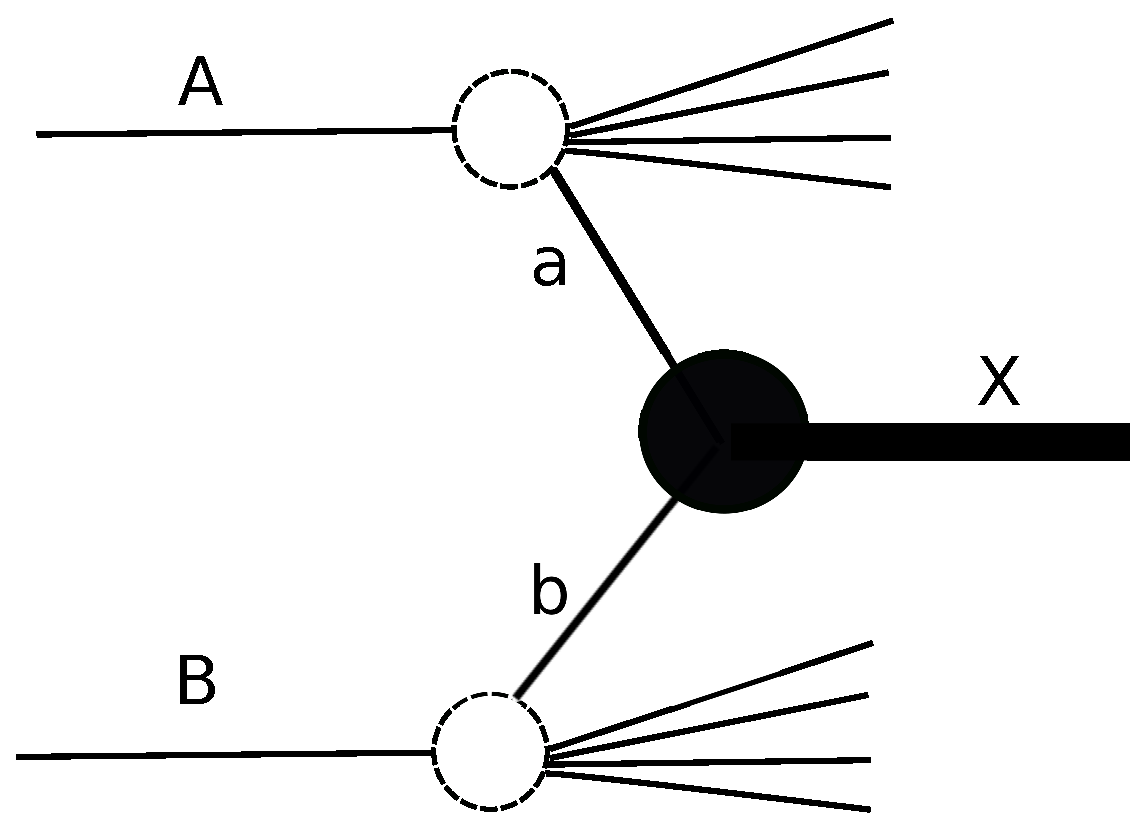
\includegraphics[width=0.6\textwidth]{figures/Theory/Hadron-Hadron.eps}
\caption[Illustration of a hadron-hadron interaction]{
Illustration showing hadron-hadron interaction through partons $a$ and $b$ going to $X$. 
\label{Theory:HadronHadron}}
\end{figure}


\subsection{Jet Formation}

From pQCD, it is expected that there is partonic emission off the final state partons, and the emission has a high probability if it is either soft or collinear. 
The resulting partons can also emit partons, and a partonic cascade occurs.
Confinement requires that all observable particles are colour neutral. 
This will only occur when there is a low relative momentum between partons.
This cascade continues until the parton's energies are at the hadronic scale, $\mathcal{O}(1\rm GeV)$, and they bond into hadrons.
The result is a cascade of hadrons in the direction of the original parton.

Calculations with partons in the final state are performed using a jet algorithm.  
The jet algorithm clusters nearby partons into a single object.
The jet algorithms can be applied to calculations at a particular order in perturbation theory, to final state hadrons, or to detector energy deposits.
Figure \ref{Theory:InitJet} shows an illustration of a jet at different levels.


\begin{figure}
\centering
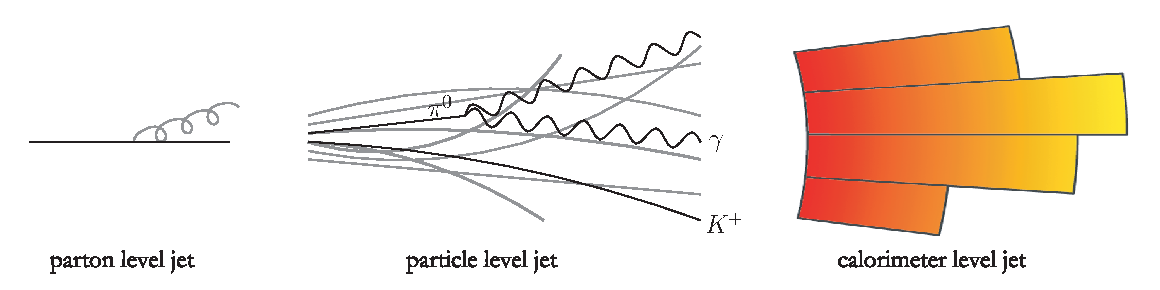
\includegraphics[width=0.9\textwidth]{figures/Theory/JetEvolution.eps}
\caption[Jets at parton, particle and calorimeter levels]{
Illustration of a jet at parton, particle and calorimeter levels. 
Illustration from Dag Gillberg.
\label{Theory:InitJet}}
\end{figure}

